%% This is file `elsarticle-template-1-num.tex',
%%
%% Copyright 2009 Elsevier Ltd
%%
%% This file is part of the 'Elsarticle Bundle'.
%% ---------------------------------------------
%%
%% It may be distributed under the conditions of the LaTeX Project Public
%% License, either version 1.2 of this license or (at your option) any
%% later version.  The latest version of this license is in
%%    http://www.latex-project.org/lppl.txt
%% and version 1.2 or later is part of all distributions of LaTeX
%% version 1999/12/01 or later.
%%
%% Template article for Elsevier's document class `elsarticle'
%% with numbered style bibliographic references
%%
%% $Id: elsarticle-template-1-num.tex 149 2009-10-08 05:01:15Z rishi $
%% $URL: http://lenova.river-valley.com/svn/elsbst/trunk/elsarticle-template-1-num.tex $
%%
\documentclass[preprint,12pt]{elsarticle}

%% Use the option review to obtain double line spacing
%% \documentclass[preprint,review,12pt]{elsarticle}

%% Use the options 1p,twocolumn; 3p; 3p,twocolumn; 5p; or 5p,twocolumn
%% for a journal layout:
%% \documentclass[final,1p,times]{elsarticle}
%% \documentclass[final,1p,times,twocolumn]{elsarticle}
%% \documentclass[final,3p,times]{elsarticle}
%% \documentclass[final,3p,times,twocolumn]{elsarticle}
%% \documentclass[final,5p,times]{elsarticle}
%% \documentclass[final,5p,times,twocolumn]{elsarticle}

%% The graphicx package provides the includegraphics command.
\usepackage{graphicx}
%% The amssymb package provides various useful mathematical symbols
\usepackage{amssymb}
%% The amsthm package provides extended theorem environments
%% \usepackage{amsthm}
\usepackage{todonotes}

%% The lineno packages adds line numbers. Start line numbering with
%% \begin{linenumbers}, end it with \end{linenumbers}. Or switch it on
%% for the whole article with \linenumbers after \end{frontmatter}.
\usepackage{lineno}

%% natbib.sty is loaded by default. However, natbib options can be
%% provided with \biboptions{...} command. Following options are
%% valid:

%%   round  -  round parentheses are used (default)
%%   square -  square brackets are used   [option]
%%   curly  -  curly braces are used      {option}
%%   angle  -  angle brackets are used    <option>
%%   semicolon  -  multiple citations separated by semi-colon
%%   colon  - same as semicolon, an earlier confusion
%%   comma  -  separated by comma
%%   numbers-  selects numerical citations
%%   super  -  numerical citations as superscripts
%%   sort   -  sorts multiple citations according to order in ref. list
%%   sort&compress   -  like sort, but also compresses numerical citations
%%   compress - compresses without sorting
%%
%% \biboptions{comma,round}

% \biboptions{}

\journal{Journal Name}

\begin{document}

\begin{frontmatter}

%% Title, authors and addresses

\title{Applying Radial Basis Networks and Markov Chains to detect concept drift in non-stationary environments}

%% use the tnoteref command within \title for footnotes;
%% use the tnotetext command for the associated footnote;
%% use the fnref command within \author or \address for footnotes;
%% use the fntext command for the associated footnote;
%% use the corref command within \author for corresponding author footnotes;
%% use the cortext command for the associated footnote;
%% use the ead command for the email address,
%% and the form \ead[url] for the home page:
%%
%% \title{Title\tnoteref{label1}}
%% \tnotetext[label1]{}
%% \author{Name\corref{cor1}\fnref{label2}}
%% \ead{email address}
%% \ead[url]{home page}
%% \fntext[label2]{}
%% \cortext[cor1]{}
%% \address{Address\fnref{label3}}
%% \fntext[label3]{}


%% use optional labels to link authors explicitly to addresses:
%% \author[label1,label2]{<author name>}
%% \address[label1]{<address>}
%% \address[label2]{<address>}

\author{Ruivaldo Neto}
\author{Adrien Brilhault}
\author{Ricardo Rios}

\address{Salvador, Brazil}

\begin{abstract}
Most real-world problems experience a phenomenon known as concept drift,
which is a change in data distribution that can affect the system performance.
%
However, the majority of drift detection methods work reactively.
These algorithms continuously monitor the system performance
and detect concept drifts when the performance drops past a threshold.
Nevertheless, some environments can not afford this deterioration in performance.
%
In an attempt to mitigate the aforementioned problem,
this paper proposes a novel proactive method for on-line drift detection,
called RBFChain.
The proposed method relies on Radial Basis Networks implicit clustering property,
besides using Markov Chains to model the transitions and for better noise tolerance.
%
To assess the proposed method as a viable concept drift detector,
an analysis of sensitivity, accuracy,
and noise tolerance was performed using synthetic datasets.
Moreover, results were compared to the most established algorithms in the literature,
demonstrating the competitivity of the method.
%
Furthermore, the algorithm was also tested with the real-world problem of eye-tracking.
This problem is relevant because many behavioral experiments use eye-tracking information (fixations and saccades) as a relevant analysis factor.
Performed experiments reveal that RBFChain can classify fixations and saccades in real-time, with high accuracy, noise tolerance, and using limited resources.

\end{abstract}

\begin{keyword}
Concept Drift \sep Drift Detection \sep Eye tracking
\end{keyword}

\end{frontmatter}

%%
%% Start line numbering here if you want
%%
\linenumbers

%% main text
\section{Introduction}
\label{sec:intro}

\todo[inline]{Add concept drift paragraph}

Eye movements are one of the most natural and repetitive motions of the human being.
Worldly activities, such as reading a book or watching television, are only possible because of these.
This regular movement, known as saccadic movement, is required by the retina to obtain a clean image.
%
During the analysis of a scene, the eye tends to fixate during a few milliseconds on the most significant areas.
After this fixation, it moves towards a new area of interest.
%
Therefore, it is possible to describe the trajectory of the eye as a sequence of fixation periods interrupted by saccades.
%
Fixation periods allow the brain to process information, given that during saccades, the brain does not have time to process the images transmitted by the visual system.
%
Hence, the brain assigns semantics to the image only during fixation periods.
Thus, the study of fixations and saccades is essential for the interpretation and understanding of the eye movements.

Most commercial eye-tracking systems provide horizontal and vertical coordinates of the point of regard (POR) relative to the screen of a monitor.
The results presented are composed of sequences of points corresponding to positions of the eyes of an individual.
The generated eye path consists of eye fixations (with a high density of points) separated by vast spaces where only a few isolated points (saccades) are present.

Automated identification of fixation and saccades is a necessary aspect in the analysis of visual behavior.
These classifications serve as underlying knowledge for the metrics used for interpreting eye movements (number of saccades, the average amplitude of saccades, number of fixations, duration of the first fixation, etc).
%
Unfortunately, the majority of the algorithms still employ a velocity, acceleration, or dispersion threshold to detect potential saccades \cite{otero:jorge:troncoso:saccades_and_fixations}.
Some techniques differ by applying additional procedures, such as principal component analysis, to distinguish between smooth search, saccades, and noise \cite{Berg2009}.
%
% One exception is the algorithm presented by \cite{Urruty:2007:DEF:1314303.1314308}, which uses dispersion
% and projection clustering into arbitrary subspace to detect fixations.

However, advances in the area of behavioral analysis have made measured eye movements more variable and complex, thus making the main methods found in the literature less effective \cite{Anderson:OneAlgorithmToRuleThemAll:2017}.

This paper proposes a novel algorithm, called RBFChain, which applies Radial Basis Function Networks and Markov Chains to classify scan paths into fixations and saccades in real-time, with high accuracy, noise tolerance, and using limited resources.
Besides that, experiments conducted in this work show that the true detection rate obtained by RBFChain is comparable to that obtained by state of the art.

The rest of the paper is organized as follows:
Section 2 describes the concept drift phenomenon and the main detection techniques;
Section 3 presents the fixations and saccades detection problem;
Section 4 describes the RBFChain algorithm and its pseudo-code;
Section 5 shows the experiment configuration for synthetic datasets  and results obtained;
Section 6 presents the examination setup with a real-world eye-tracking problem and observed outcomes; and, finally, Section 7 provides conclusions
and discusses future work.

\section{Concept Drift}
\label{sec:concept_drift}

Most real-world problems experience a phenomenon known as
concept drift \cite{Gama:2014:DAF:2670967.2670971}.
This situation happens in datasets where the
joint probability distribution changes arbitrarily over time, such as a switch in the conditional probability distribution on a classification problem, or a change of some moment (such as mean and variance) on a time series forecasting problem \cite{tsymbal2004problem}.

Environments that generate this kind of data are considered non-stationary.
In these environments, concepts tend to evolve frequently, and the system may be unable to adapt to the new information, hence dramatically deteriorating its performance.
%
Many relevant real-world problems can be considered as non-stationary environments.
Examples include financial market monitoring, telecom networks, intruder detection, spam filtering, among others \cite{Gama:2014:DAF:2670967.2670971}.

In the literature, Bayesian Theory is commonly used as a background to define the concept drift phenomenon formally \cite{Elwell:2011}: consider the posterior probability of a sample $x$ belonging to a class $y$, a concept drift happens when this probability changes over time, that is, $Pt + 1 (y | x) \neq Pt (y | x)$. In a supervised learning scenario, this can be interpreted as when the relationship between the input data and the target variable change over time.

According to \cite{tsymbal2004problem, Gama:2014:DAF:2670967.2670971}, concept drifts can occur in four main patterns:

\begin{itemize}
    \item \textbf{Abrupt:} occurs when a concept A switches abruptly to another concept B.
    \item \textbf{Gradual:} occurs when a concept A is being exchanged for the B concept gradually. In this case, while there is no definitive change from concept A to concept B, occurrences of B become more frequent, while fewer events of A are observed.
    \item \textbf{Incremental:} occurs when a concept A is being exchanged for B through intermediate concepts.  These concepts differ little from its predecessor and successor. So changes are noticeable only in the long run.
    \item \textbf{Recurrent:} occurs when a previously active concept reappears after a certain period. However, this can not be understood as a periodic seasonality.
\end{itemize}

Figure \ref{fig:concept_drift_patterns} demonstrates these patterns:

\begin{figure}[h!]
\begin{center}
    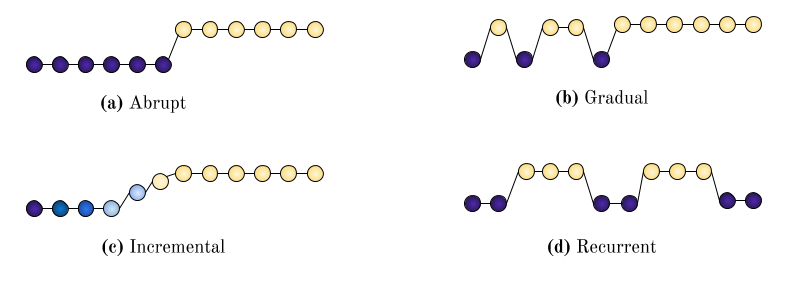
\includegraphics[scale=0.65]{img/concept_drift_patterns.png}
    \caption{Concept Drift Patterns}
    \label{fig:concept_drift_patterns}
\end{center}
\end{figure}

Algorithms for detecting concept drift characterize and quantify concept drifts through the delimitation of the moments or time intervals in which changes occur \cite{Basseville:1993:DAC:151741}.
%
These algorithms fall into two categories, according to the need for data labeling \cite{Zliobaite:2010}:

\begin{itemize}
    \item \textbf{Explicit Algorithms/Supervised}: These methods adopt a passive approach, as they depend on the correct labeling of the data to act. The model performance is monitored continuously, and drifts are detected when its performance starts to deteriorate, reaching a threshold.
    \item \textbf{Implicit Algorithms/Unsupervised:} These algorithms take a proactive approach and are independent of correct data labeling. Concept drifts are detected through the analysis of incoming data or indicators produced by the applied learning techniques. Although they are more prone to false alarms, they are an alternative to scenarios where obtaining labels is expensive, time-consuming or unviable. Also, this approach can lead to better results, since it is possible to refit the model or adjust the data, before the deterioration of the predictions.
\end{itemize}

The algorithm proposed in this paper classifies itself as an unsupervised algorithm and adopts a proactive approach.
Briefly, its operation can be described: The Radial Basis Function Networks continuously cluster all incoming data.
Changes in the generated cluster (a different center is activated) reflect in a Markov Chain, which keeps an online model of the possible system transitions and its probabilities. Drifts are triggered when the transition probability reaches a parametric threshold.

To assess the proposed method as a viable concept drift detector, an analysis of sensitivity, accuracy, and noise tolerance was performed using synthetic datasets. Moreover, results were compared to the most established algorithms in the literature, demonstrating the competitivity of the method.

\section{Fixations and Saccades detection}
\label{sec:eye_tracking}

Visual perception involves six types of eye movements \cite{leigh2015neurology}, among which fixations and saccades are the most relevant.
During fixation, the eye is kept relatively stable on an area of interest (AOI). In contrast, saccades are fast eye movements enabling the fovea to fixate different regions of the scene \cite{privitera:2005:scanpath_theory}.
Thus, the process of looking at a scene can be represented by a sequence of fixations and saccades, the so-called visual scan path.
Research on scan path analysis and visual perception has benefited from the recent development of eye trackers.
Today’s eye-tracking systems allow a precise recording of eye movements at high sampling rates, thus enabling a detailed analysis of the viewing behavior.

Despite recent advances, reliable automated clustering of eye movements is still challenging, even more so in dynamic scenarios.
In many applications, e.g., human-computer gaze-based interaction, driving assistance systems, online adaptation of digital content based on gaze analysis, the identification of fixations and saccades has to occur in an online fashion.
There is a wide variety of methods for the online analysis of eye-tracking data and the recognition of fixations and saccades.
However, only a few of them are suited for online applicability to dynamic scenes.
Such methods have to quickly adapt not only to the individual viewing behavior but also to the changes occurring in the viewing scene.
This small group of highly promising methods is based on probabilistic formalizations, e.g.,
as Markov Models \cite{Salvucci:2000:IFS:355017.355028, Komogortsev2013},
Bayesian Mixture Models \cite{Tafaj:2012:BOC:2168556.2168617}, etc.

Prior techniques for the automated recognition of different types of eye movements from eye-tracking data fall into two main categories:
(i) threshold-based methods, where the distinction of fixations from saccades is based on dispersion, velocity, or acceleration thresholds, and
(ii) probabilistic methods. These groups of techniques will be briefly discussed in the following.

Threshold-based methods distinguish between fixations and saccades based on the assumption that the distances, velocities, or accelerations occurring between subsequent fixations differ from those occurring between saccades.
The goal then is to identify a threshold based on which saccades can be reliably distinguished from fixations.

When distance thresholds are used, fixation clusters are usually identified by searching for data points that are close enough to each other (i.e., below the established threshold) within a predefined time window \cite{holmqvist-eye-tracking-a-comprehensive-guide-to-methods-and-measures}.
A representative of this group, is the Dispersion Threshold Identification (I-DT) algorithm \cite{Salvucci:2000:IFS:355017.355028}.
Other similar approaches differ mainly in the way the threshold is calculated \cite{Blignaut2009, Shic:2008:IFM:1344471.1344500}.

Other algorithms in this realm are based on the computation of Minimum Spanning Trees (MST).
In \cite{Salvucci:2000:IFS:355017.355028} an MST is built on the eye-tracking points within a temporal window of predefined length.
An edge (i.e., representing the distance between two points) is classified as a saccade if its length is significantly larger than the lengths of neighboring edges,
which have been previously classified as distances between fixations.
Yet other methods employ smart clustering algorithms, e.g., \cite{Santella:2004:RCE:968363.968368, Urruty:2007:DEF:1314303.1314308}
but have serious limitations concerning their applicability to dynamic online scenarios,
since, in such scenarios, the cluster properties for fixations and saccades show high variability.

Methods that are based on velocity or acceleration thresholds work similarly.
A representative of this group is the Velocity-Threshold Identification (I-VT) algorithm,
where a point is identified as a saccade point,
if the implicit velocity along the distance from the previous data point to that point exceeds a predefined threshold.
Otherwise the data point is assigned to a fixation cluster \cite{Salvucci:2000:IFS:355017.355028}.

In summary, the major drawback of threshold-based methods is that they rely on thresholds that have to be empirically adjusted to the individual viewing behavior,
the viewing area, and the specific task.
Each of these parameters can have significant influence on the classification result \cite{Komogortsev2013, Salvucci:2000:IFS:355017.355028}.
For this reason and because of the fact that the viewing behavior is strongly physically and physiologically-dependent, such methods are not reliable, especially when real-time analysis of eye-tracking data is needed.

Probabilistic methods are built on soft decision rules, which are formalized as probabilities, e.g.,  the probability of a data point being a saccade given the previous observations. The probabilities – and thus, the decisions – are adjusted to the observations.

One of the most prominent probabilistic methods applied to the identification of fixations and saccades is the Hidden Markov Model (HMM).
An HMM is a simple dynamic Bayesian network with variables representing values from a discrete state and observation space.
The state of a variable represents the class of the current observation. It is only dependent on the state (i.e., class of the previous observation).
Because of this sequential nature, such models are a popular choice for the analysis of successively arising data points (i.e., observations).
For the detection of fixations and saccades from eye data, HMMs have been used with velocity observations between successive data points,
thus allowing the adaptation of the model to the physiological viewing behavior \cite{Salvucci:2000:IFS:355017.355028}.
In the model of \cite{Salvucci:2000:IFS:355017.355028} (coined I-HMM),
the two states used represent discretized velocity distributions over fixations and saccades.
Transition probabilities between the states represent the probability of the current sample belonging to a fixation cluster or a saccade,
given the previous state \cite{holmqvist-eye-tracking-a-comprehensive-guide-to-methods-and-measures}.
Due to the above probabilistic representation, no thresholds are needed.
The I-HMM is reported to outperform fixed-threshold methods,
such as I-VT \cite{Salvucci:2000:IFS:355017.355028}.
In summary, the sequential, dynamic,
and probabilistic nature of HMMs makes them an adequate choice for data arising in an online fashion and containing variability in its features.

Probabilistic mixture models, such as the Bayesian Mixture Model (BMM) presented in \cite{Tafaj:2012:BOC:2168556.2168617},
build on the assumption that the observed data is generated from a mixture of unknown density distributions.
The goal is to estimate the parameters of these distributions based on observed data points and to derive the most probable distribution that might have generated a given data point.

The algorithm presented in \cite{Tafaj:2012:BOC:2168556.2168617} could distinguish between fixations and saccades in an online fashion,
only by considering the Euclidean distances between subsequent data points.
The underlying model is based on the assumption
that distances between subsequent fixation points will, in general, be shorter than distances between subsequent saccade points;
that is, distances between subsequent fixation points would be generated from a specific Gaussian distribution and those between subsequent saccade points from another.
This intuition was modeled by a Bayesian Online Mixture Model.
The benefit of the Bayesian formalization of the mixture model
is that the parameters of the two distributions are updated and learned in an online fashion as more and more data is observed.
For every new data point, the prior probabilities are replaced by the latest estimates.
For practical purposes, this means that for every new user the algorithm needs a relatively small number of data points to
adjust to that user and learn user- or scene-dependent parameters.

In summary, probabilistic methods come with three main advantages over threshold-based ones:

\begin{enumerate}
    \item No fixed thresholds are needed. Instead, the parameters of the model (e.g., state transition probabilities, label emission probabilities, and other settings) are learned from labeled data.
    \item Both HMMs and BMMs can adapt to the individual (i.e., physiological) viewing behavior of a subject and the specific task.
    \item Given the dynamic nature of the underlying models, the methods are naturally suited for data arising in an online fashion, such as eye-tracking data.
\end{enumerate}

\section{RBFChain algorithm}
\label{sec:rbfchain_algorithm}

This section details the RBFChain implementation. However, before describing the proposed method, it is significant to present the main applied concepts of Radial Base Function Networks and Markov Chains.

\subsection{Radial Basis Function Networks (RBFN)}

Radial Basis Function Networks (RBFN) are used in various disciplines with a reasonable degree of success. The broad applicability is a result of their excellent ability to make function approximation, especially when the relationships among the variables of interest are nonlinear \cite{Bishop:2006:PRM:1162264}.

A radial basis function network is a type of artificial neural network (ANN), and most neural networks are known to be useful in modeling complex and nonlinear relationships. An RBFN has advantages in specific applications in that for a given parameter set, RBFN networks do not require an iterative procedure to learn the model. Iterative learning for most ANN types is computationally expensive and vulnerable to the local minima problem.

The topology of an RBFN is given in Fig. \ref{fig:rbg_arq} as a multiple input single output feedforward network.
Assume that there are $n$ input variables labeled from $x_1$ to $x_n$.
The network receives input samples as vectors $x=(x_1, x_2, \ldots, x_n)$ of size $1 \times n$.
The initial layer is only a buffer that feeds the input values to the intermediate layer, which is called the hidden layer.
There are $n_h$ processing elements in the hidden layer.
Each processing element in the hidden layer processes the input vector and produces a single value output. This processing is performed through a basis function $\phi$.
Finally, the output layer weights the results of the intermediate layer by weights, aggregating them linearly to compose the final network response.

Among many candidates for basis functions, Gaussian radial basis function (RBF), presented in Eq. \ref{eq:gaussian}, is used in this study. The main reason for this choice is that it can be shown that an RBFN with Gaussian RBF can sufficiently approximate any given function for a large enough number of hidden layer elements \cite{Theodoridis:2008:PRF:1457541}.

Probabilistic methods are built on soft decision rules, which are formalized as probabilities, e.g.,  the probability of a data point being a saccade given the previous observations. The probabilities – and thus, the decisions – are adjusted to the observations.


\begin{equation}
    \label{eq:gaussian}
    \varphi (v_{i})=e^{-(\sigma r)^{2}}
\end{equation}

In the hidden layer, each processing element has a separate vector called the center, which has the same dimensions as the input vector.
For $n_h$ hidden layer elements we have $n_h$ center vectors as $(c_1; c_2; \ldots; {c_n}_h)$.
Then each processing element looks at the distance between the input vector and its center and uses this distance to create its output (activation phase).


This work uses only the initial and intermediary layers of the presented architecture.
The initial layer channels the incoming data to the middle layer, which implicitly forms clusters during the activation phase.
The formed grouping has an active center that changes according to the processed value.
Changes in the active center are interpreted as possible concept drifts.

\begin{figure}[h!]
\begin{center}
    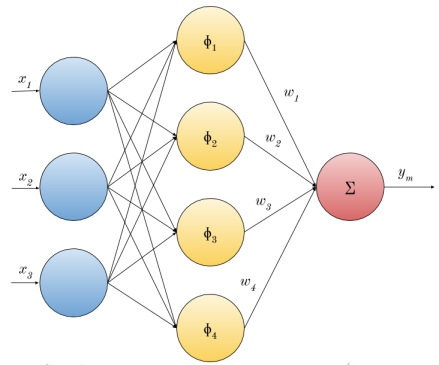
\includegraphics[scale=0.75]{img/rbf_arq.png}
    \caption{Topology of a RBFN}
    \label{fig:rbg_arq}
\end{center}
\end{figure}


\subsection{Markov Chains}

A Markov chain model can be defined by the tuple $(S; A; \lambda)$. S corresponds to the state space, A is a matrix representing transition probabilities from one state to another, and $\lambda$ is the initial probability distribution of the states in S. If there are $n$ states in our Markov chain, then the
matrix of transition probabilities $A$ is of size $n \times n$.

The fundamental property of the Markov model is the dependency on the previous state. If the vector $s(t)$ denotes the probability vector for all the states at time $t$, then:

\begin{equation}
    \label{eq:markov}
    \hat { s } ( t ) = \hat { s } ( t - 1 ) A
\end{equation}

In this proposal, Markov chains are used to model the transitions (activations) between centers in the Radial Basis Function Network.
For this formulation, a Markov state corresponds to one of the centers.

When the RBFN identifies a different center, a new state is registered in the Markov Chain.
Initially, all possible transitions from this center have a zero value.
If another center is activated, this change produces an increment in the probability of the correspondent transition.
In paralell, all other transitions probabilites are decreased proportionally to the total number of possible transitions.

The use of a Markov Chain allows the proposed algorithm to keep an online model of the transitions. The probabilities sustained in this model are compared to parametric thresholds, to indicate when a warning zone is triggered, or a concept drift happens.

\subsection{RBFChain}

\ldots

\section{Analyses on Synthetic Datasets with Concept Drift}
\label{sec:results_synthetic_dataset}

\subsection{Experimental Setup}

\subsection{Results}

\section{Detection of Saccade and Fixation}
\label{sec:detection_of_saccade_and_fixation}

\subsection{Experimental Setup}

\subsection{Results}

\section{Concluding Remarks}

\bibliographystyle{model1-num-names}
\bibliography{references}

\end{document}

%%
%% End of file `elsarticle-template-1-num.tex'.